\section{Context and Overview}
\label{sec:back}
\vspace{10pt}

%big picture overview of tenant-side decision-making, where PMaaS fits within this, mention the specific assumptions we make, the chosen environment, which ideas are likely to generalize to other settings
 
\begin{figure*}%[htbp]
\centering
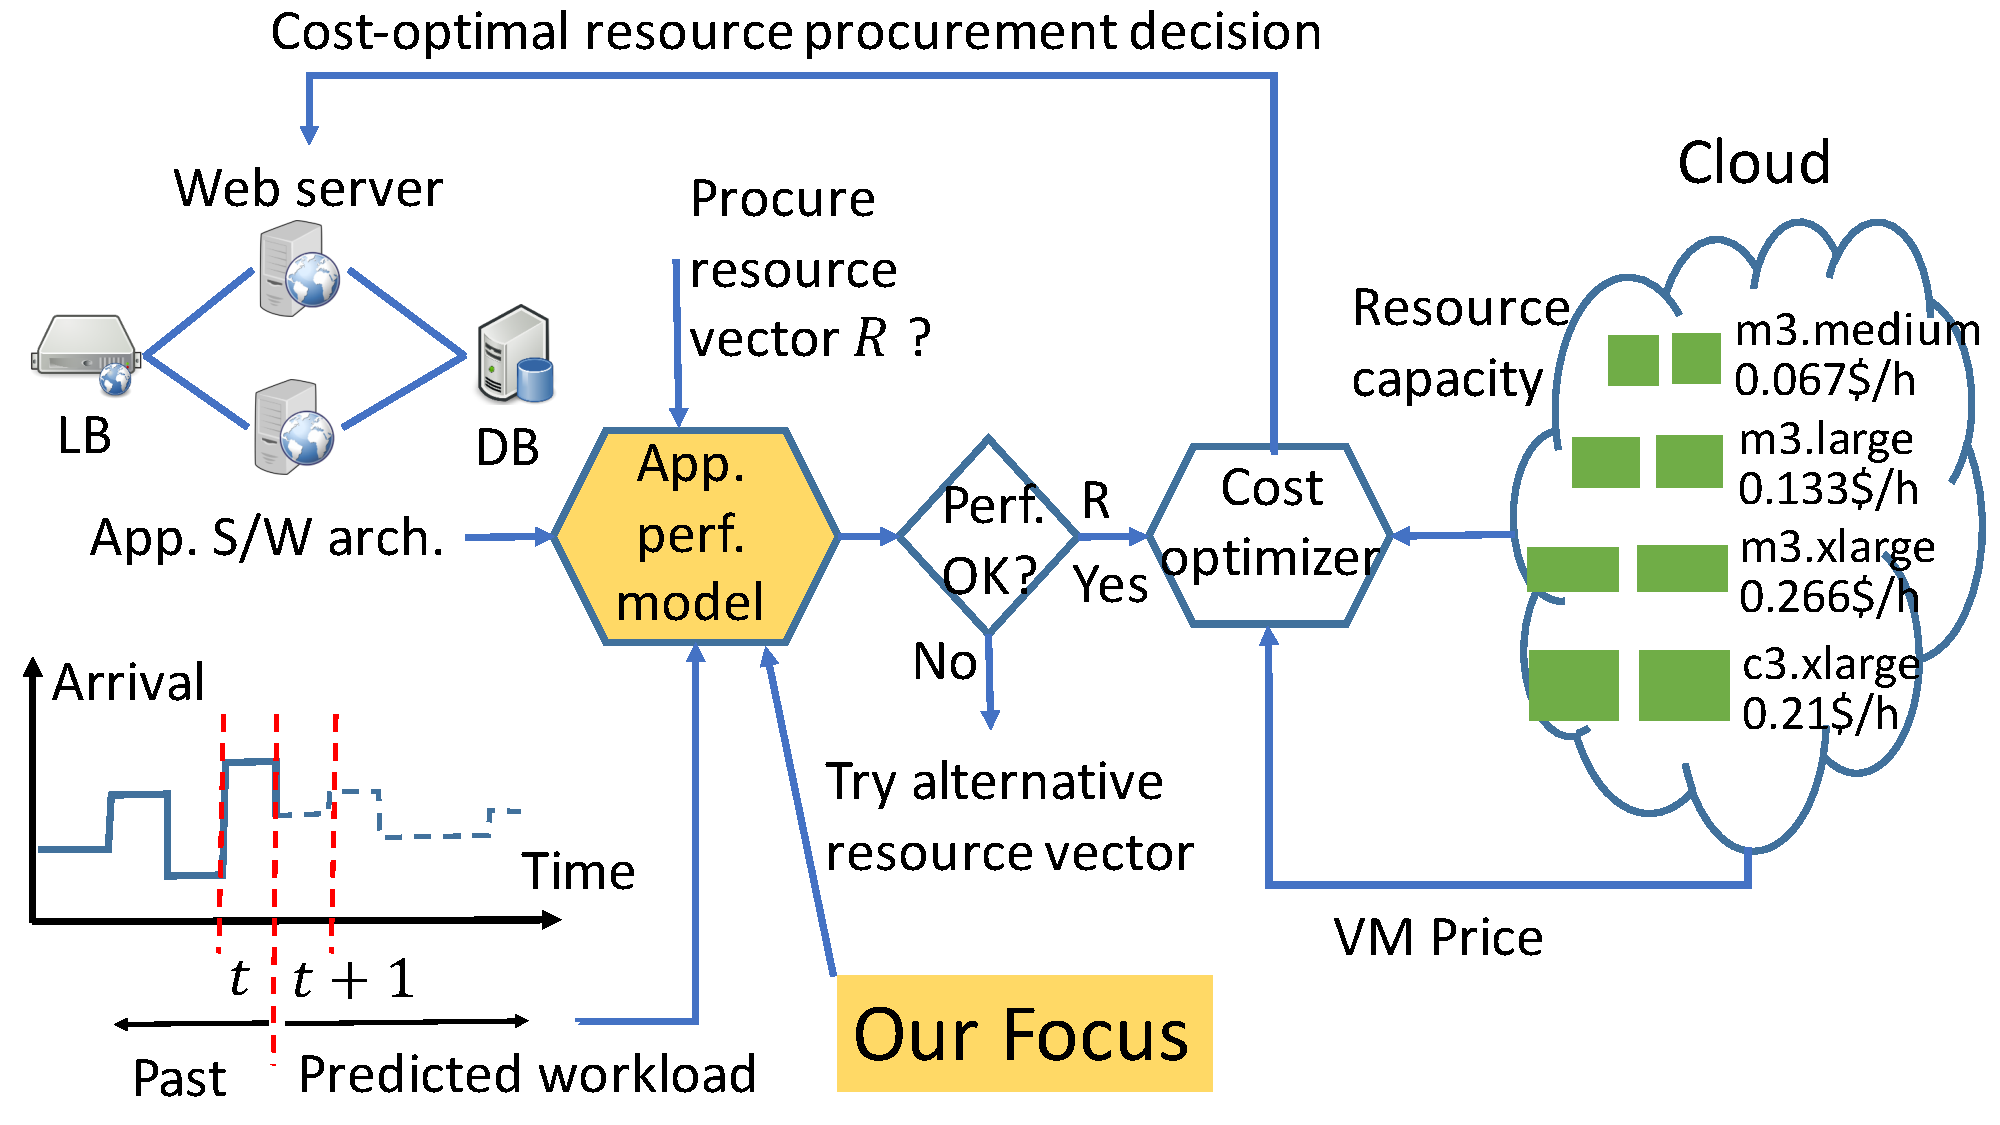
\includegraphics[width=0.8\textwidth]{system}
\caption{An overview of interactions between the performance modeling problem we study and other aspects of the overall decision-making for a cost-conscious tenant procuring resources from a public cloud. }
\label{fig:diagram}
%\vspace{-10pt}
\end{figure*}

Figure~\ref{fig:diagram} shows the essential elements making up the decision-making that a general cost-conscious tenant might carry out when procuring resources from a public cloud. In particular, it clarifies the role of application performance modeling within this overall decision-making and its interaction with other elements. 
%** expand this, 
The tenant would employ observations of its workload intensity in the past to predict its future workload. Consider the example of a key-value store or a database application that we employ in our evaluation in Section~\ref{sec:eval}. Such an application might keept track of request arrival rates (possibly for different request classes) and then use a suitable prediction mechanism for estimating future arrival rate. Whereas some tenant applications exhibit significant predictability (e.g., captured well via Markovian or autoregressive models)~\cite{xxx}, others are known to exhibit poor predictability and must resort to short-term (``myopic'') estimates~\cite{xxx}. Regardless, having made these predictions, the tenant must then ascertain the number and type of VMs that it must procure from the cloud to meet its performance needs (or deallocate from its existing resource pool). 

%Figure~\ref{fig:diagram} shows 
We show one way of thinking about this decision-making~\footnote{The actual realization of this overall decision-making may be different from how we describe it here. Our description is deliberately designed to highlight the role of the application performance model.}, wherein the tenant determines (using its application performance model) multiple VM allocation choices that would allow it to meet its predicted workload with the requisite performance goals. These choices are then compared in terms of their costs (or expected profits, if the tenant wishes to maximize expected profits rather than minimizing costs) via an optimization problem that incororates idiosyncrasies of the prices offered by the public cloud. Finally, the most cost-effective choice identified by the optimizer is used as the basis for actually procuring the appropriate number and type of VMs from the cloud provider. 

%**point to related work, repeat that our arguments are not tied to a particular modeling technique. **
Significant research exists both on predicting workloads and on performance modeling (see Section~\ref{sec:related}) for a wide variety of application types. Recall that our interest in this paper is not on devising new techniques for workload prediction or application performance modeling. Rather, we are interested in evaluating the role VM diversity might play in calibrating a {\it given} performance model. Towards this, we next describe one popularly used modeling approach that we adapt for our purposes. 

%what about the costs of PMaaS itself? how to make it practical? might providers actually offer it as a service?
